\chapter{Mathematical Description of the Project}
\label{Ch:mathematical description}
For an automated trading robot with reinforcement learning, investment decisions and actions are made periodically. We allocate fixed amount of budget into two stocks, aiming to maximize return while controlling the volatility and considering the transaction cost. These are the mathematical setting of the portfolio management problem.

\section{Mathematical Formalism}
We define $p_1,p_2,p_3,...,p_t,...$ as the close price of an stock sequences of each day released from the exchange center. Then for another stock, its close price sequence is $q_1,q_2,q_3,...,q_t,...$. Let price vector to be $(p_t, q_t)$. We use price price change vector $(\frac{p_t-p_t-1}{p_t-1},\frac{q_t-q_t-1}{q_t-1})$ to define the state later.
$pv_t$ is the portfolio value at time period t, which is calculated based on the market value of two stocks and two stocks' weight. We define $a_t$ as weight of stock1 at the time period t in the portfolio value. It is calculated as the proportion of stock1's market value in the total portfolio value.We define the initial portfolio as \$ 10,000 which is called budget from now on.



\section{Transaction Cost}
In a real world, buying or selling stocks is not free. The cost includes commission fee, tax, etc. Assuming a transaction cost proportional to the stock market values exchanged in the market, we set the rate to be 0.2\%. We used the preceding study by Angelos to determine the rate. Since we assumed the stock share to be float type, we used formula below to calculate transaction cost. 
$$\frac{T}{2} = |\frac{pv_t}{p_t}a_{t-1} - \frac{pv_{t+1}-T}{p_t+1}a_t|*p_t*rate$$


\section{Benchmark}
The model’s test data performance was compared against two benchmarks. We used the preceding study by Oliver and Hamza to determine the benchmarks. The first, the do-nothing benchmark, allocates half of its starting budget to each stock half-half and then does nothing. This benchmark acted as a very crude approximation of the market since it represents the raw performance of the two stocks.

The second, the rebalance benchmark, re-evaluates its holdings at the end of every market days, and buys or sells stock to ensure the total portfolio value is split into 50-50 between the two stocks. It is important to note that it maintains a proportion of stock values, not stock shares.

\section{Dataset and Features}
We trained our Q-table and neural network using historical stock data gathered from Yahoo finance using the Python library Pandas.DataReader to automatically download the stock histories. 

Stock riskiness is quantified by beta index. Beta bigger than 1 indicates that a stock is more volatile than the market, while less volatile stock has a beta smaller than 1. We chose ten stocks from S \& P 500’s high-beta index fund, and five low-beta stocks from 2000/05/01 to 2001/05/01. Then we random choose two high-beta stock from those ten, and one low-beta stock from those five to make up two stock pairs for test. For the other thirty two possible combination made up by the remained stocks, we randomly chose ten pairs to train our model. 

For testing, we also chose two stocks combination based on beta index. We tested on two combinations in order to reduce the impact of the unique behavior of the data. We used AMAT(1.29) and CAJ(0.78), and FCX(2.53) and CAJ(0.78) as test sets. 

\begin{figure}[h]
\begin{center}
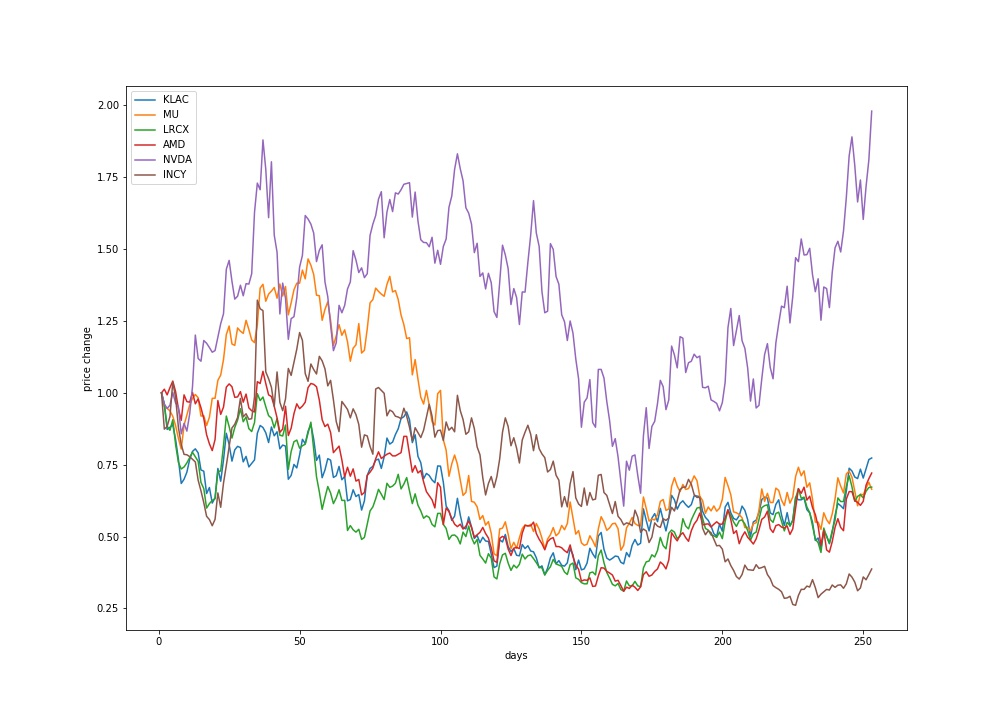
\includegraphics[clip, width=0.6\textwidth]{Graphics/highbeta_pricechange.jpg} \caption{High Beta Stock}
\end{center}
\end{figure}

\begin{figure}[h]
\begin{center}
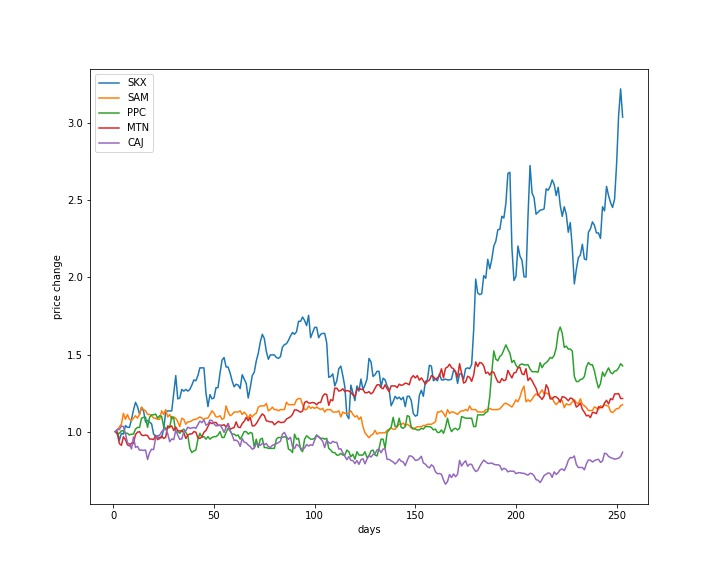
\includegraphics[clip, width=0.6\textwidth]{Graphics/lowbeta_pricechange.jpg} \caption{Low Beta Stock}
\end{center}
\end{figure}

\section{Assumption}
While building model for portfolio management, we took some assumptions. First, we buy and sell the stock at the close price. Second, our behavior of buying and selling does not affect the stock market. Third, we can discretize the stock price and the stock unit to be bought and sell can be non-integer. Lastly, transaction rate occurred by buying and selling are same, and proportional to the exchanged market value.	
